\documentclass{beamer}
\usetheme{Antibes}
\useinnertheme{rectangles}
\useoutertheme{infolines}
\usepackage[utf8]{inputenc}
\usepackage[T1]{fontenc}
\usepackage{graphicx}

% Patch the look of +, = in arev
\usefonttheme{serif}

\usepackage{arev}
% Patch punctuation to be upright
\DeclareMathSymbol{.}{\mathpunct}{operators}{`.}
\DeclareMathSymbol{,}{\mathpunct}{operators}{`,}

\usepackage{amsmath}
\usepackage{amssymb}

\setbeamertemplate{footline}{%
\begin{beamercolorbox}[ht=3.0ex,dp=1ex]{title in head/foot}
\hfill\footnotesize\insertpagenumber\enspace\enspace\end{beamercolorbox}}

\definecolor{bluegreen1}{rgb}{0.0,0.20,0.28}
\definecolor{bluegreen2}{rgb}{0.0,0.20,0.28}
\setbeamercolor*{palette primary}{fg=white,bg=bluegreen1}
\setbeamercolor*{palette secondary}{fg=white,bg=bluegreen2}
\setbeamercolor*{palette tertiary}{fg=white,bg=bluegreen2}
\setbeamercolor{itemize item}{fg=black}
\setbeamercolor{block title}{bg=bluegreen2}
\newcommand{\modest}[1]{{\small\color{gray}#1}}

\newcommand{\ee}{\mathrm e}
\newcommand{\ui}{\mathrm i}
\newcommand{\real}{\operatorname{Re}}
\newcommand{\imag}{\operatorname{Im}}
\newcommand{\uv}[1]{\underline{#1}}
\newcommand{\bv}[1]{\mathbf{#1}}

\newcommand{\N}{\mathbb N}
\newcommand{\Z}{\mathbb Z}
\newcommand{\Q}{\mathbb Q}
\newcommand{\R}{\mathbb R}
\newcommand{\C}{\mathbb C}

\newcommand{\id}{\operatorname{id}}
\newcommand{\sgn}{\operatorname{sgn}}
\newcommand{\Abb}{\operatorname{Abb}}
\newcommand{\unit}[1]{\mathrm{#1}}
\newcommand{\chem}[1]{\mathrm{#1}}
\newcommand{\strong}[1]{\textsf{\textbf{#1}}}

\title{Was ist Ableiten?}
\date{}

\begin{document}
\maketitle

%\begin{frame}[t]
%\frametitle{Inhaltsverzeichnis}
%\tableofcontents
%\end{frame}

\begin{frame}

\begin{Definition}
Ableitung von $f$ an der Stelle $x$:
\[f'(x) := \lim_{h\to 0}\frac{f(x+h)-f(x)}{h}.\]
\end{Definition}

\end{frame}


\begin{frame}
Was bedeutet das?
\end{frame}

\begin{frame}
Beim Ableiten approximiert man den Graph einer Funktion an einer
Stelle $x_0$ durch eine Gerade. Die Definition der Ableitung ist
gerade die Berechnungsvorschrift, mit der man den Anstieg $a=f'(x_0)$
dieser Geraden erhält.
\end{frame}

\begin{frame}
\begin{center}
\includegraphics[width=0.8\textwidth]{img/Ableitung.pdf}
\end{center}
\end{frame}

\begin{frame}
Man kann doch gleich auch eine beliebige Kurve $\gamma\colon\R\to\R^2$
an einem Punkt mit einer Geraden approximieren?
\end{frame}

\begin{frame}
Ja, klar. Alles was wir brauchen ist eine Berechnungsvorschrift,
die der Kurve den Richtungsvektor der Geraden zuordnet:
\begin{block}{Ableitung einer Kurve}
\[\gamma'(t) = \lim_{h\to 0}\frac{\gamma(t+h)-\gamma(t)}{h}\]
\end{block}
\end{frame}

\begin{frame}
Eigentlich muss man die gewöhnliche Ableitung nur Komponentenweise
berechnen:
\[\begin{aligned}\gamma'(t) &= \lim_{h\to 0} \frac{
\begin{bmatrix}\gamma_x(t+h)\\ \gamma_y(t+h)\end{bmatrix}
-\begin{bmatrix}\gamma_x(t)\\ \gamma_y(t)\end{bmatrix}}{h}\\
& = \lim_{h\to 0}
\begin{bmatrix}\frac{\gamma_x(t+h)-\gamma_x(t)}{h}\\
\frac{\gamma_y(t+h)-\gamma_y(t)}{h}\end{bmatrix}
= \begin{bmatrix}\gamma_x'(t)\\ \gamma_y'(t)\end{bmatrix}.
\end{aligned}\]
\end{frame}

\begin{frame}
Oder, um es banaler auszudrücken, einfach mit dem Differentialoperator
$D=\mathrm d/\mathrm dt$ ausmultiplizieren:
\[D\gamma = D(\gamma_x\mathbf e_x+\gamma_y\mathbf e_y)
= \mathbf e_x D\gamma_x+\mathbf e_y D\gamma_y.\]
Die Basisvektoren $\mathbf e_x,\mathbf e_y$ dürfen als konstante
Faktoren angesehen und vor die Ableitung gezogen werden.

\end{frame}

\begin{frame}
\begin{center}
\includegraphics[width=0.6\textwidth]{img/Tangentialvektor.pdf}
\end{center}
\end{frame}

\begin{frame}
\textbf{Einwand.}
Aber eine Oberfläche $f\colon\R\times\R\to\R$ wird doch auch durch
eine Tangentialebene approximiert? Was ist da denn der Anstieg
oder die Richtung?
\end{frame}

\begin{frame}
Eine Ebene ist durch
\[E(x,y) = f(x_0,y_0)+a(x-x_0)+b(y-y_0)\]
gegeben. Hält man jetzt $y:=y_0$ konstant, dann ergibt sich eine
Gerade
\[g(x) = f(x,y_0)+a(x-x_0)\]
mit dem Anstieg $a$. Es gibt also je Variable einen Anstieg. Diese
Anstiege sind die partiellen Ableitungen.
\end{frame}

\begin{frame}
Wir können die Ebenengleichung mittels Skalarprodukt kompakter schreiben:
\[E(x,y) = f(x_0,y_0) + \langle\begin{bmatrix}a\\ b\end{bmatrix},
\begin{bmatrix}x-x_0\\ y-y_0\end{bmatrix}\rangle\]
\end{frame}

\begin{frame}
Der Vektor
\[(\nabla f)(x_0,y_0) := \begin{bmatrix}(\partial_x f)(x_0,y_0)\\ (\partial_y f)(x_0,y_0)\end{bmatrix}
= \begin{bmatrix}a\\ b\end{bmatrix}\]
heißt \emph{Gradient} von $f$ an der Stelle $(x_0,y_0)$, wobei $\partial_x f$
und $\partial_y f$ die partiellen Ableitungen sind.
\end{frame}

\begin{frame}
Fassen wir doch auch die Koordinaten $x,y$ zu einem Koordinatentupel $\mathbf x = (x,y)$
zusammen. Die Gleichung der Ebene lautet nun
\[E(\mathbf x) = f(\mathbf x_0) + \langle(\nabla f)(\mathbf x_0),\mathbf x-\mathbf x_0\rangle,\]
was ganz analog zu
\[g(x) = f(x_0) + f'(x_0)(x-x_0)\]
ist.
\end{frame}

\begin{frame}
\textbf{Einwand.}
Aber der Definitionsbereich der Fläche $f(x,y)$ kann doch einfach ein
affiner Raum sein? Auf einem affinen Raum ist doch nicht unbedingt ein
Skalarprodukt definiert? Trotzdem ergibt doch der Gedanke einen Sinn,
dass $f(x,y)$ durch eine Ebene approximiert werden kann?
\end{frame}

\begin{frame}
Ja. Das Skalarprodukt ist hier in Wirklichkeit eine duale Paarung aus
einem Kovektor mit einem Vektor. Der Gradient
\[(\nabla f)(x_0,y_0) = (\partial_x f)(x_0,y_0)\mathbf e_x + (\partial_y f)(x_0,y_0)\mathbf e_y\]
muss gegen das Differential
\[(\mathrm df)(x_0,y_0) = (\partial_x f)(x_0,y_0)\mathrm dx + (\partial_y f)(x_0,y_0)\mathrm dy\]
ausgetauscht werden. Das Differential ist der Kovektor.
Die Differentiale $\mathrm dx$ und $\mathrm dy$
sind die Basisvektoren der Dualbasis zu $(\mathbf e_x,\mathbf e_y)$.
\end{frame}

\begin{frame}
Duale Paarung?
\end{frame}

\begin{frame}
Das ist fast banal. Bei einer dualen Paarung eines Kovektors
$\omega=\omega_x\mathrm dx+\omega_y\mathrm dy$ mit
einem Vektor $\mathbf v = v_x\mathbf e_x+v_y\mathbf e_y$ darf man einfach
das Standardskalarprodukt auf die Komponententupel anwenden, auch
wenn $B=(\mathbf e_1,\mathbf e_2)$ keine Orthonormalbasis ist.
Duale Paarung:
\[\omega(\mathbf v) = \omega_x v_x+\omega_y v_y.\]
\end{frame}

\begin{frame}
Bei der Differenz $\mathbf v=\mathbf x-\mathbf x_0$ handelt es sich nicht
um einen Punkt, sondern um einen Verschiebungsvektor, der den Punkt
$\mathbf x_0$ zu $\mathbf x$ verschiebt: $\mathbf x_0+\mathbf v = \mathbf x$.
Die Gleichung der Ebene nimmt nun die folgende allgemeine Form an:
\[E(\mathbf x) = f(\mathbf x_0) + (\mathrm df)(\mathbf x_0)(\mathbf x-\mathbf x_0).\]
\end{frame}

\begin{frame}
\textbf{Einwand.} Aber einer Parameterfläche $F(u,v)$ mit
$F\colon\R^2\to\R^3$ kann man doch auch eine Tangentialebene zuordnen?
\end{frame}

\begin{frame}
Die partielle Ableitung lässt sich Komponentenweise berechnen.
Insgesamt ergibt sich ein Tangentialvektor. Die beiden
Tangentialvektoren $(\partial_u F)(u_0,v_0)$ und $(\partial_v F)(u_0,v_0)$
bilden dann eine Tangentialbasis des Tangentialraums. Der
\emph{Tangentialraum}, das ist wenn man die Tangentialebene als
Vektorraum betrachtet.
\end{frame}

\begin{frame}
\begin{center}
\includegraphics[width=0.6\textwidth]{img/Tangentialebene.pdf}
\end{center}
\end{frame}

\begin{frame}
Die Tangentialvektoren lassen sich nach Wahl eines
Koordinatensystems als Komponententupel betrachten und
zur Jacobimatrix
\[DF = \begin{bmatrix}
\partial_u F_x & \partial_v F_x\\
\partial_u F_y & \partial_v F_y\\
\partial_u F_z & \partial_v F_z
\end{bmatrix}\]
zusammenfassen.
\end{frame}

\begin{frame}
Ist $F\colon\R^n\to\R^m$, dann lässt sich $F$ an der Stelle
$\mathbf u_0$ linear durch einen Tangentialraum approximieren.
Die Approximation besitzt die Berechnungsvorschrift
\[T(\mathbf u) = F(\mathbf u_0)+(DF)(\mathbf u_0)(\mathbf u-\mathbf u_0),\]
was wieder ganz analog zu
\[g(x) = f(x_0)+f'(x_0)(x-x_0)\]
ist. Mit $(DF)(\mathbf u_0)\in\R^{m\times n}$ ist die Jacobimatrix
gemeint.
\end{frame}

\begin{frame}
Aber eine Matrix ist doch nichts anderes als die Darstellungsmatrix
einer linearen Abbildung bezüglich einer Basis. Warum müssen wir eine
Basis wählen?
\end{frame}

\begin{frame}
Klar, wir müssen natürlich keine Basis wählen und können die
Ableitung $(DF)(\mathbf u_0)$ als lineare Abbildung betrachten. Beachte aber
dass eine lineare Abbildung immer eine Abbildung zwischen zwei
Vektorräumen ist.\\[1em]
Die Differenzen $\mathbf u-\mathbf u_0$ sind wie gesagt Vektoren.
Sie gehören zum Definitionsbereich der linearen Abbildung. Und die
Zielmenge der linearen Abbildung? Die ist ebenfalls ein Vektorraum,
für den bisher auch immer eine Basis gewählt wurde, denn es war
jedes mal der Koordinatenraum.
\end{frame}

\begin{frame}
\textbf{Einwand.} Bei einer Kurve beschreibt der Richtungsvektor
den Tangentialraum. Bei einer Funktion muss die Funktion doch
erst als Kurve betrachtet werden?
\end{frame}

\begin{frame}
Ja richtig, die Bildmenge der linearen Abbildung ist nur dann
der Tangentialraum, wenn eine Parameterdarstellung eines krummen
geometrischen Objektes vorliegt.
\end{frame}

\begin{frame}
\textbf{Einwand.}
Und wenn bei $F\colon M\to N$ die Definitionsmenge und die Zielmenge
selbst so eine krumme Oberfläche ist? Dann ist das doch am Ursprung
$\mathbf u_0$ kein Vektorraum mehr, und $\mathbf u-\mathbf u_0$ ergibt
keinen sind mehr! Trotzdem wird man irgendwie den Gedanken nicht los,
dass $F$ trotzdem irgendwie \emph{smooth} sein könnte, so dass sich
die Ableitung bilden lässt.
\end{frame}

\begin{frame}
Huch? Was machen wir jetzt? Nun, die Ableitung soll die Approximation
von $F$ durch eine lineare Abbildung sein. Aber die muss immer
zwischen zwei Vektorräumen bestehen. Es ist doch irgendwie sinnvoll,
dafür an der Stelle $p=\mathbf u_0$ den Tangentialraum $T_p M$ und
am Bildpunkt $F(p)$ den Tangentialraum $T_{F(p)}N$ zu wählen,
so dass $F$ eine lineare Abbildung zwischen diesen beiden
Tangentialräumen ist.
\end{frame}

\begin{frame}
Ja. Ernsthaft. Wenn wir dann mit einem Vektor $v$ geringfügig von
der Stelle $p=\mathbf u_0$ wegschieben, dann lässt sich mit
der linearen Abbildung eine Approximation der Funktion berechnen,
deren Wert im Tangentialraum zu $F(p)$ liegt.
\end{frame}

\begin{frame}
Ok. Also $F\colon M\to N$ ist eine Funktion zwischen zwei
glatten Mannigfaltigkeiten. Weil $M$ glatt ist, gibt es zu jedem
Punkt $p\in M$ den Tangetialraum $T_p M$. Und den Tangentialraum
$T_{F(p)}N$ gibt es ebenfalls. Die Funktion $F$ lässt sich nun
in der Nähe vom Punkt $p$ durch die lineare Abbildung
\[(\mathrm dF)(p)\colon T_pM\to T_{F(p)}N\]
approximieren.
\end{frame}

\begin{frame}
Man bezeichnet die Ableitung $(\mathrm dF)(p)$ auch als das
Differential von $F$ an der Stelle $p$. Die Applikation auf einen
Vektor $v$ wird auch \emph{Pushforward} von $v$ genannt.
Die Vorstellung dabei ist, dass $v$
von $T_pM$ vorwärts zu $T_{F(p)}N$ gepusht wird.
\end{frame}

\begin{frame}
Äh? Die Ableitung soll doch einen Tangentialraum beschreiben.
Warum werden die denn jetzt vorausgesetzt?
\end{frame}

\begin{frame}
Wenn man $F$ tatsächlich als Parameterdarstellung eines krummen
geometrischen Objektes betrachtet, dann beschreibt die Bildmenge
der linearen Abbildung $(\mathrm dF)(p)$ tatsächlich den
Tangentialraum $T$ des Objetes am Punkt $F(p)$. Offenbar ist
$T\subseteq T_{F(p)}N$. D.\,h. $T$ darf ein Untervektorraum
von $T_{F(p)}N$ sein.
\end{frame}

\begin{frame}
\begin{center}
\includegraphics[width=0.8\textwidth]{img/Differential.pdf}
\end{center}
\end{frame}

\begin{frame}
Wenn wir für eine differenzierbare Mannigfaligkeit $M$ eine Karte
haben (so wie die Karten der Erdoberfläche), das ist eine diffeomorphe
Abbildung
\[\varphi\colon (U\subseteq \R^n)\to V\subseteq M,\]
dann lässt sich $\varphi$ als gekrümmtes Koordinatensystem auf $M$
betrachten. Die partiellen Ableitungen $(D_k\varphi)(\mathbf x_0)$ sind
Tangentialvektoren von $M$ am Punkt $p=\varphi(\mathbf x_0)$.
Die Tangentialvektoren bilden die Tangentialbasis, das ist ein lokales
ungekrümmtes Koordinatensystem, welches das gerümmte Koordinatensystem
bei $p$ approximiert. 
\end{frame}

\begin{frame}
Die disjunkte Zusammenfassung aller Tangentialbasen wird als
\emph{Rahmen} bezeichnet. Die Karte $\varphi$ induziert diesen
Rahmen, und der Rahmen induziert das Tangentialbündel $TM$, weil
man für jeden Punkt $p\in M$ den Tangentialraum $T_pM$ aus der Basis
aufspannen kann, wobei die Information über die Basis verloren geht.
\end{frame}

\begin{frame}
Aber die Ableitung einer Karte $\varphi$ ist doch auch so ein
komischer Pushforward?
\end{frame}

\begin{frame}
Ja, $(\mathrm d\varphi)(\mathbf x_0)$ ist eine lineare Abbildung,
die jedem $v=\mathbf x-\mathbf x_0$ einen Tangentialvektor
\[w = (\mathrm d\varphi)(\mathbf x_0)(v)\]
mit $w\in T_pM$ und $p=\varphi(\mathbf x_0)$ zuordnet.
\end{frame}

\begin{frame}
Eine Karte $\varphi$ induziert als Diffeomorphismus an der Stelle
$\mathbf x\in\R^n$ eine injektive lineare
Abbildung $(\mathrm d\varphi)(\mathbf x)$, deren Koordinatendarstellung die
Jacobimatrix
\[(D\varphi)(\mathbf x)\colon\R^n\to\R^m\]
ist.
Die Jacobimatrix muss nicht quadratisch sein, hat aber den Rang $n$,
ordent also einer Basis des $\R^n$ eine Basis des $n$-dimensonalen
Tangentialraums zu.
\end{frame}

\begin{frame}
Eigentlich sollte die lineare Abbildung bijektiv sein und eine quadratische
Matrix besitzen, aber dann müsste
man einen Rahmen für die Bildmenge von $\varphi$ wählen. Der Rahmen
wird jedoch erst durch $\mathrm d\varphi$ erzeugt.
\end{frame}

\begin{frame}
Ok, der $\R^n$ ist doch der Koordinatenraum. Dort liegt doch die
Standardbasis $\mathrm E=(\mathbf e_k)_{k=1}^n$ vor. Bsp.
$\mathbf e_1=(1,0)$ und $\mathbf e_2=(0,1)$. Dann ist
\[\mathbf w_k = (\mathrm d\varphi)(\mathbf x_0)(\mathbf e_k)\]
die induzierte Basis von $T_pM$ bei $p=\varphi(\mathbf x_0)$.
\end{frame}

\begin{frame}
Warum induziert $\varphi$ eine injektive lineare Abbildung?
\end{frame}

\begin{frame}
Wenn $\varphi$ diffeomorph ist, sind $\varphi$ und $\varphi^{-1}$
differenzierbar. Dann gilt die Kettenregel:
\[\mathrm{id} = \mathrm d(\varphi^{-1}\circ\varphi)(\mathbf x)
= \mathrm d\varphi^{-1}(\varphi(\mathbf x))\circ\mathrm d\varphi(\mathbf x).\]
In Worten: $\mathrm d\varphi^{-1}(\varphi(\mathbf x))$ ist die
Linksinverse von $\mathrm d\varphi(\mathbf x)$. Somit muss
$\mathrm d\varphi(\mathbf x)$ injektiv sein.
\end{frame}

\begin{frame}
Ende.
\vfill\hfill\modest{Juli 2020}\\
\hfill\modest{Creative Commons CC0 1.0}
\end{frame}


\end{document}


